\documentclass{article}

\usepackage[romanian]{babel}

\usepackage{graphicx} % Required for inserting images
\usepackage[a4paper, margin=1in]{geometry}
\usepackage{parskip}
\usepackage[most]{tcolorbox}
\usepackage{tabularx}
\usepackage[table,xcdraw]{xcolor}
\usepackage{array}
\usepackage{multirow}
\usepackage[utf8]{inputenc}
\usepackage{multicol}

\graphicspath{ {.} }

\usepackage{listings}
\usepackage{tcolorbox}
\tcbuselibrary{listingsutf8}

% Define Java language
\lstdefinelanguage{Java}{
  morekeywords={abstract,assert,boolean,break,byte,case,catch,char,class,const,
    continue,default,do,double,else,enum,extends,final,finally,float,for,if,
    implements,import,instanceof,int,interface,long,native,new,package,private,
    protected,public,return,short,static,strictfp,super,switch,synchronized,this,
    throw,throws,transient,try,void,volatile,while},
  morecomment=[l]{//},
  morecomment=[s]{/*}{*/},
  morestring=[b]",
  sensitive=true
}

% Define a tcolorbox environment for Java code
\newtcblisting{javacodebox}[1][]{%
  colback=white!5!white, % Background color
  colframe=violet!75!black, % Frame color
  title=#1, % Title for the box (optional)
  fonttitle=, % Title font
  listing only,
  listing options={%
    language=Java,
    basicstyle=\ttfamily\small, % Font style and size
    keywordstyle=\color{blue}, % Style for keywords
    commentstyle=\color{green!60!black}, % Style for comments
    stringstyle=\color{red!70!black}, % Style for strings
    tabsize=2, % Tab width
    showstringspaces=false,
    breaklines=true, % Automatic line breaking
    frame=none,
  },
  enhanced,
  breakable,
  boxrule=0.5mm, % Thickness of the frame
  arc=1mm, % Rounded corners
}


\setlength{\parskip}{.5em}

\title{MIPS32 Pipeline Simulator}
\author{Bogdan Marcu}
\date{October 2024}

\begin{document}

\maketitle

\newpage

\tableofcontents

\newpage
\section{Introduction}
\subsection{Context}
The project aims to provide a \textbf{MIPS} (\textbf{M}icroporcessor Without \textbf{I}nterlocked \textbf{P}ipeline \textbf{S}tages) with pipeline 32-bit architecture simulator software. The pipeline architecture, in the context of CPU design, consists of splitting the execution stages of an instruction across different levels, which can run concurrently, thus achieving better performance.This architecture, presents many advantages, such as increasing clock frequency by significantly reducing the critical path in instruction execution, therefore obtaining a better throughput, or out of order execution. However, this architecture substantially raises the complexity of the CPU. 

The Simulator plans on enabling the user to intuitively visualize how a sequence of instructions would execute on the MIPS32 Pipeline CPU, displaying detailed information for each stage of the pipeline for teaching or debugging purposes.
\subsection{Objectives}
The simulator will be implemented in Java, with the user interface being developed using web technologies, specifically the Next.js framework. The UI will enable the user to analyze the execution of instructions in each of the pipeline stages, including, but not limited to viewing the value of the pipeline stage registers, relevant flag information, such as branch/jump flags, arithmetical logical unit operation codes and memory or register files contents.   
\newpage
\section{Bibliographic Research}

\subsection{Description of the MIPS Pipeline Architecture}
The single cycle MIPS architecture is made of multiple instruction processing stages that contribute to the complete and correct execution of an instruction in a one clock cycle. Given this, the period of a clock cycle must last for at least as long as the delay introduced by the hardware components for the longest instruction, called the critical path, causing a performance bottleneck.

To address this limitation, a pipeline architecture for the MIPS processor was introduced. It consists of multiple registers interposed between each two of the instruction execution stages - Instruction Fetch, Instruction Decode, Execute, Write Back - and enables for multiple instructions to be processed at the same time but in different sections of the pipeline. This not only dramatically reduces the critical path in the CPU, leading to faster operating clock speeds, but also paves the way for implementing hardware optimization techniques such as branch prediction or out of order execution.

\subsection{Simulating concurrent behaviour in sequential programs}
Simulating concurrent behavior in sequential programs, such as a MIPS pipeline simulator in Java, involves mimicking the parallel execution of tasks within a single-threaded environment. In a MIPS pipeline, multiple instructions are processed simultaneously at different stages (e.g., fetch, decode, execute, memory access, write-back), but a sequential program like Java cannot truly run these in parallel. To simulate concurrency, we implement the stages in a way that they appear to be running concurrently.

The general principle for achieving concurrent-like behaviour within a sequential program is component synchronization using an event based architecture, which will be elaborated comprehensively in the next sections. The core idea consists of components being controlled by a bootstrapper higher level component that is aware of the order in which each of the components should operate and dispatches them as soon as it is notified that the previous pipeline stage has finished work or when they are due.

\newpage
\section{Analiză}

\subsection{Analiza proiectului}
Simulatorul MIPS Pipeline va dispune de următoarele capabilități:
\begin{enumerate}
    \item User Interface - will give the user the possibility to see:
    \begin{itemize}
        \item The contents of every stage register
        \item The contents of the instruction memory
        \item The value of the Program Counter
        \item Decoded information about the current instruction
        \item The Contents of the Register File
        \item ALU current operation, operand and result
        \item Memory content
    \end{itemize}
    \item The user will be able to toggle between auto-ticking and manual ticking modes of the clock
    \item The following 32-bit instructions will be supported:
    \begin{enumerate}
        \item add, addi - addition between registers, register and immediate
        \item sub - subtraction between registers
        \item sll, srl - shift right, left logical
        \item and, or, xor - bit-wise logical operation
        \item lw - load word from memory
        \item sw - store word to memory
        \item beq - branch on equal
        \item bgtz - branch on greater than zero
        \item bne - branch on not equal
        \item noop - operation that has no effect - used for hazard solving
        \item jump - jump to instruction
    \end{enumerate}
\end{enumerate}

\subsection{Interfața grafică}
\label{subsec:ui}
Interfața grafică a simulatorului are ca scop simplificarea modului în care utilizatorul simulatorului interacționează cu sistemul. Astfel, în interiorul acesteia, se regăsește o schemă bloc care cuprinde toate elementele de interes pentru scopul acestui proiect din interiorul procesorului. Aceasta va cuprinde toate etajele de execuție ale procesorului, cu componentele acestora, precum blocuri de registre, blocuri de memorie, unități de execuție, dar și registrele dintre etaje. Toate acestea vor furniza utilizatorului, în timp real, datele ce sunt în curs de procesare în pipeline.

De asemenea, prin intermediul interfeței grafice, utilizatorul va putea încărca cod în limbaj de asamblare pentru a-l rula în simulator. Codul va fi validat pentru eventuale erori, iar apoi încărcat în memoria de program a procesorului virtual. Mai departe, utilizatorul va putea porni simularea execuției, fie pas cu pas, declanșând manual fiecare front de ceas, ceea ce permite un timp de analiză extins după nevoie, fie cu derulare automată a semnalului de ceas, la un interval de timp selectat.

\subsection{Generarea de cod mașină din instrucțiuni}
Simulatorul este capabil sa genereze cod mașină, pe care, apoi, să îl ruleze pe procesorul virtual, pornind de la instrucțiunile în limbaj de asamblare suportate. Astfel, simulatorul trebuie sa fie capabil de a valida, interpreta și traduce instrucțiunile introduse de utilizator în mod corect si eficient. În cazul unor erori de sintaxă, precum greșeli de tip \textit{typo}, folosiresa unor instrucțiuni invalide, folosirea unor operanzi invalizi, sau utilizarea unui format incorect al unui tip de instrucțiune, acesta va produce erori și nu va permite execuția acestora, prevenind eventual comportament netereminist.

\begin{tcolorbox}[colback=blue!5!white,colframe=violet!75!black,title=Cazuri de validare]
    \begin{enumerate}
        \item Numele instrucțiunii este invalid
        \item Formatul instrucțiunii nu corespunde cu tipul acesteia
        \begin{enumerate}
            \item numărul operanzilor este altul decât cel așteptat
        \end{enumerate}
        \item Operanzii sunt invalizi
        \begin{enumerate}
            \item Formatul operanzilor este incorect
            \item Tipul de dată diferă față de cel așteptat
            \item Dimensiunea operanzilor nu se află în limitele permise
            \item Sunt folosiți operanzi nepermiși pentru instrucțiunea curentă (ex. folosirea registrului \$0 ca registru destinație)
        \end{enumerate}
    \end{enumerate}
\end{tcolorbox}

\label{subsec:intro}
\subsection{Simularea execuției}
Proiectul urmărește simularea arhitecturii MIPS Pipeline cât mai aproape de comportamentul real. Astfel, aplicația simulează individual fiecare etaj al liniei de execuție a procesorului și asigură sincronizarea corecta între componente, respectând ordinea de execuție în care acestea trebuie să ruleze. Execuția poate avea loc în mod secvențial, în care utilizatorul declanșează manual fiecare semnal de ceas, sau automat, în care acesta doar o declanșează la momentul dorit, urmând să ruleze până când este oprita.

\begin{tcolorbox}[colback=white!5!white,colframe=violet!75!black,title=Cazuri de utilizare]
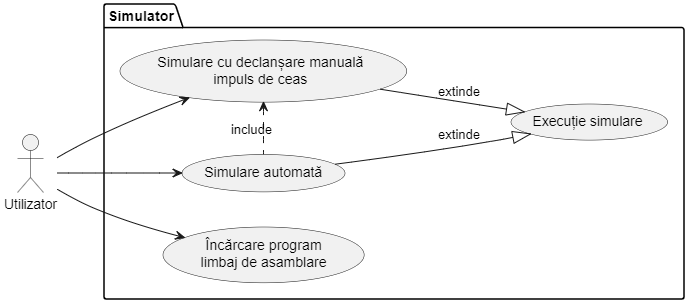
\includegraphics[scale=0.80]{img/UseCaseDiagram.png}
\end{tcolorbox}

\subsection{Instrucțuni}
\label{subsec:instr}
Simulatorul executa toate cele 3 tipuri de instrucțiuni MIPS, cu format pe 32 de biți. Astfel, instrucțiunile vor fi de unul dintre cele trei tipuri: 
\begin{enumerate}
    \item \textbf{Tip R} - Instrucțiuni a căror ambi operanzi sunt regiștrii.
        \begin{table}[ht]
        \arrayrulecolor{violet!75!black}
            \begin{tabularx}{\linewidth}{XXXXXX}
                \hline
                \rowcolor{blue!5!white}
                \multicolumn{1}{|c|}{OpCode} & \multicolumn{1}{c|}{RS} & \multicolumn{1}{c|}{RT} & \multicolumn{1}{c|}{RD} & \multicolumn{1}{c|}{SA} & \multicolumn{1}{c|}{Func} \\ \hline
                31 \hfill 26 & 25 \hfill 21 & 20 \hfill 16 & 15 \hfill 11 & 10 \hfill 6 & 5 \hfill 0 \\ 
            \end{tabularx}
        \end{table}

        Operația este de forma RD $ \leftarrow $ RS (op) RT
        \begin{itemize}
            \item OpCode = 0 pentru toate instrucțiunile de acest tip
            \item RS - Registru sursă 
            \item RT - Registru target
            \item RD - Registrul destinație
            \item SA - Dimensiunea deplasării în cazul operațiilor de deplasare pe biți
            \item Func - Codul de identificare instrucțiunii. Este necesar datorită OpCode = 0
        \end{itemize}
    \item \textbf{Tip I} - Instrucțiuni cu un operand de tip registru și un operand de tip valoare imediată.
        \begin{table}[ht]
        \arrayrulecolor{violet!75!black}
            \begin{tabularx}{\linewidth}{
                >{\hsize=.333\hsize\linewidth=\hsize}X
                >{\hsize=.333\hsize\linewidth=\hsize}X
                >{\hsize=.333\hsize\linewidth=\hsize}X
                >{\hsize=1\hsize\linewidth=\hsize}X
            }
                \hline
                \rowcolor{blue!5!white}
                \multicolumn{1}{|c|}{OpCode} & \multicolumn{1}{c|}{RS} & \multicolumn{1}{c|}{RT} & \multicolumn{1}{c|}{Immediate/Offset}\\ 
                \hline
                31 \hfill 26 & 25 \hfill 21 & 20 \hfill 16 & 15 \hfill 0 \\ 
            \end{tabularx}
        \end{table}
        
        Operația este de forma RT $ \leftarrow $ RS (op) Immediate
        \begin{itemize}
            \item OpCode - Codul instrucțiunii
            \item RS - Registru sursă 
            \item RT - Registru target
            \item Immediate/Offset - Operandul imediat sau deplasamentul, în cazul instrucțiunilor de branch
        \end{itemize}
    \item \textbf{Tip J} - Instrucțiuni de salt
        \begin{table}[ht]
        \arrayrulecolor{violet!75!black}
            \begin{tabularx}{\linewidth}{
                >{\hsize=.3\hsize\linewidth=\hsize}X
                >{\hsize=1.7\hsize\linewidth=\hsize}X
            }
                \hline
                \rowcolor{blue!5!white}
                \multicolumn{1}{|c|}{OpCode} & \multicolumn{1}{c|}{Address}\\ 
                \hline
                31 \hfill 26 & 25 \hfill 0\\ 
            \end{tabularx}
        \end{table}

        \begin{itemize}
            \item OpCode - Codul instrucțiunii
            \item Address - Adresa la care se va face saltul 
        \end{itemize}
\end{enumerate}

\arrayrulecolor{black}

\begin{tcolorbox}[colback=white!5!white,colframe=violet!75!black,title=Instrucțiuni suportate]

\begin{tabularx}{\linewidth}{|c|c|X|X|}
\hline
\multicolumn{1}{|l|}{Tip} & Instrucțiune & Sintaxă & RTL Abstract \\ \hline
\multirow{11}{*}{R} & add & add \$rd, \$rs, \$rt & RF{[}rd{]} ← RF{[}rs{]} + RF{[}rt{]} \\ \cline{2-4} 
 & sub & sub \$rd, \$rs, \$rt & RF{[}rd{]} $\leftarrow$ RF{[}rs{]} - RF{[}rt \\ \cline{2-4} 
 & sll & sll \$rd, \$rs, \$rt & RF{[}rd{]} $\leftarrow$ RF{[}rs{]} $<<$ RF{[}rt{]} \\ \cline{2-4} 
 & srl & srl \$rd, \$rs, \$rt & RF{[}rd{]} $\leftarrow$ RF{[}rs{]} $>>$ RF{[}rt{]} \\ \cline{2-4} 
 & and & and \$rd, \$rs, \$rt & RF{[}rd{]} $\leftarrow$ RF{[}rs{]} \& RF{[}rt{]} \\ \cline{2-4} 
 & or & or \$rd, \$rs, \$rt & RF{[}rd{]} $\leftarrow$ RF{[}rs{]} \| RF{[}rt{]} \\ \cline{2-4} 
 & xor & xor \$rd, \$rs, \$rt & RF{[}rd{]} $\leftarrow$ RF{[}rs{]} \oplus RF{[}rt{]} \\ \cline{2-4} 
 & beq & beq \$rt, \$rs, offset & \begin{tabular}[c]{@{}l@{}}\textbf{if} RF{[}\$rs{]} = RF{[}rt{]} \textbf{then}\\{       }PC = PC + 1 + $S_{Ext}$(offset)\\ \textbf{else}\\ {      }PC = PC + 1 \end{tabular} \\ \cline{2-4} 
 & bgtz & bgtz \$rs, offset &  \begin{tabular}[c]{@{}l@{}}\textbf{if} RF{[}\$rs{]} $>$ 0 \textbf{then}\\{       }PC = PC + 1 + $S_{Ext}$(offset)\\ \textbf{else}\\{      }PC = PC + 1\end{tabular}\\ \cline{2-4} 
 & bne & bne \$rt, \$rs, offset & \begin{tabular}[c]{@{}l@{}}\textbf{if} RF{[}\$rs{]} = RF{[}RT{]} \textbf{then}\\{      }PC = PC + 1\\ \textbf{else}\\{       }PC = PC + 1 + $S_{Ext}$(offset)\end{tabular} \\ \cline{2-4} 
 & noop & noop &  \\ \hline
\multicolumn{1}{|l|}{\multirow{4}{*}{I}} & addi & addi \$rt, \$rs, imm & RF{[}rt{]} $\leftarrow$ RF{[}rs{]} + $S_{Ext}$(imm)  \\ \cline{2-4} 
\multicolumn{1}{|l|}{} & subi & subi \$rt, \$rs, imm & RF{[}rt{]} $\leftarrow$ RF{[}rs{]} - $S_{Ext}$(imm)  \\ \cline{2-4} 
\multicolumn{1}{|l|}{} & lw & lw \$rt, \$rs, imm & RF{[}rt{]} $\leftarrow$ MEM[RF{[}rs{]} + $S_{Ext}$(imm)] \\ \cline{2-4} 
\multicolumn{1}{|l|}{} & sw & sw \$rt, \$rs, imm & MEM[RF{[}rs{]} + $S_{Ext}$(imm)] $\leftarrow$ RF{[}rt{]} \\ \hline
\multicolumn{1}{|l|}{J} & jump & jmp imm &  PC $\leftarrow$ Ext(Imm)\\ \hline
\end{tabularx}
\end{tcolorbox}

\newpage
\section{Proiectare}
\subsection{Arhitectură generală}
La nivel înalt, arhitectura unui procesor MIPS Pipeline este formată din mai multe etaje de execuție: IF (\textbf{I}nstruction \textbf{F}etch), ID (\textbf{I}nstruction \textbf{D}ecode), EX (\textbf{Ex}ecution Unit), MEM(\textbf{Mem}ory), WB (\textbf{W}rite \textbf{B}ack). Procesul de execuție al unei instrucțiuni parcurge, în general, toate aceste etape pentru a produce efectul dorit. Simulatorul ce este descris în acest document urmărește, la nivel structural, arhitectura procesorului propriu-zis. Astfel, fiecare etaj al pipeline-ului are o componenta echivalentă în arhitectura simulatorului. Diagrama de clase prezentată în cele ce urmează ilustrează această arhitectură.

\begin{tcolorbox}[colback=white!5!white,colframe=violet!75!black,title=Diagrama de clase]
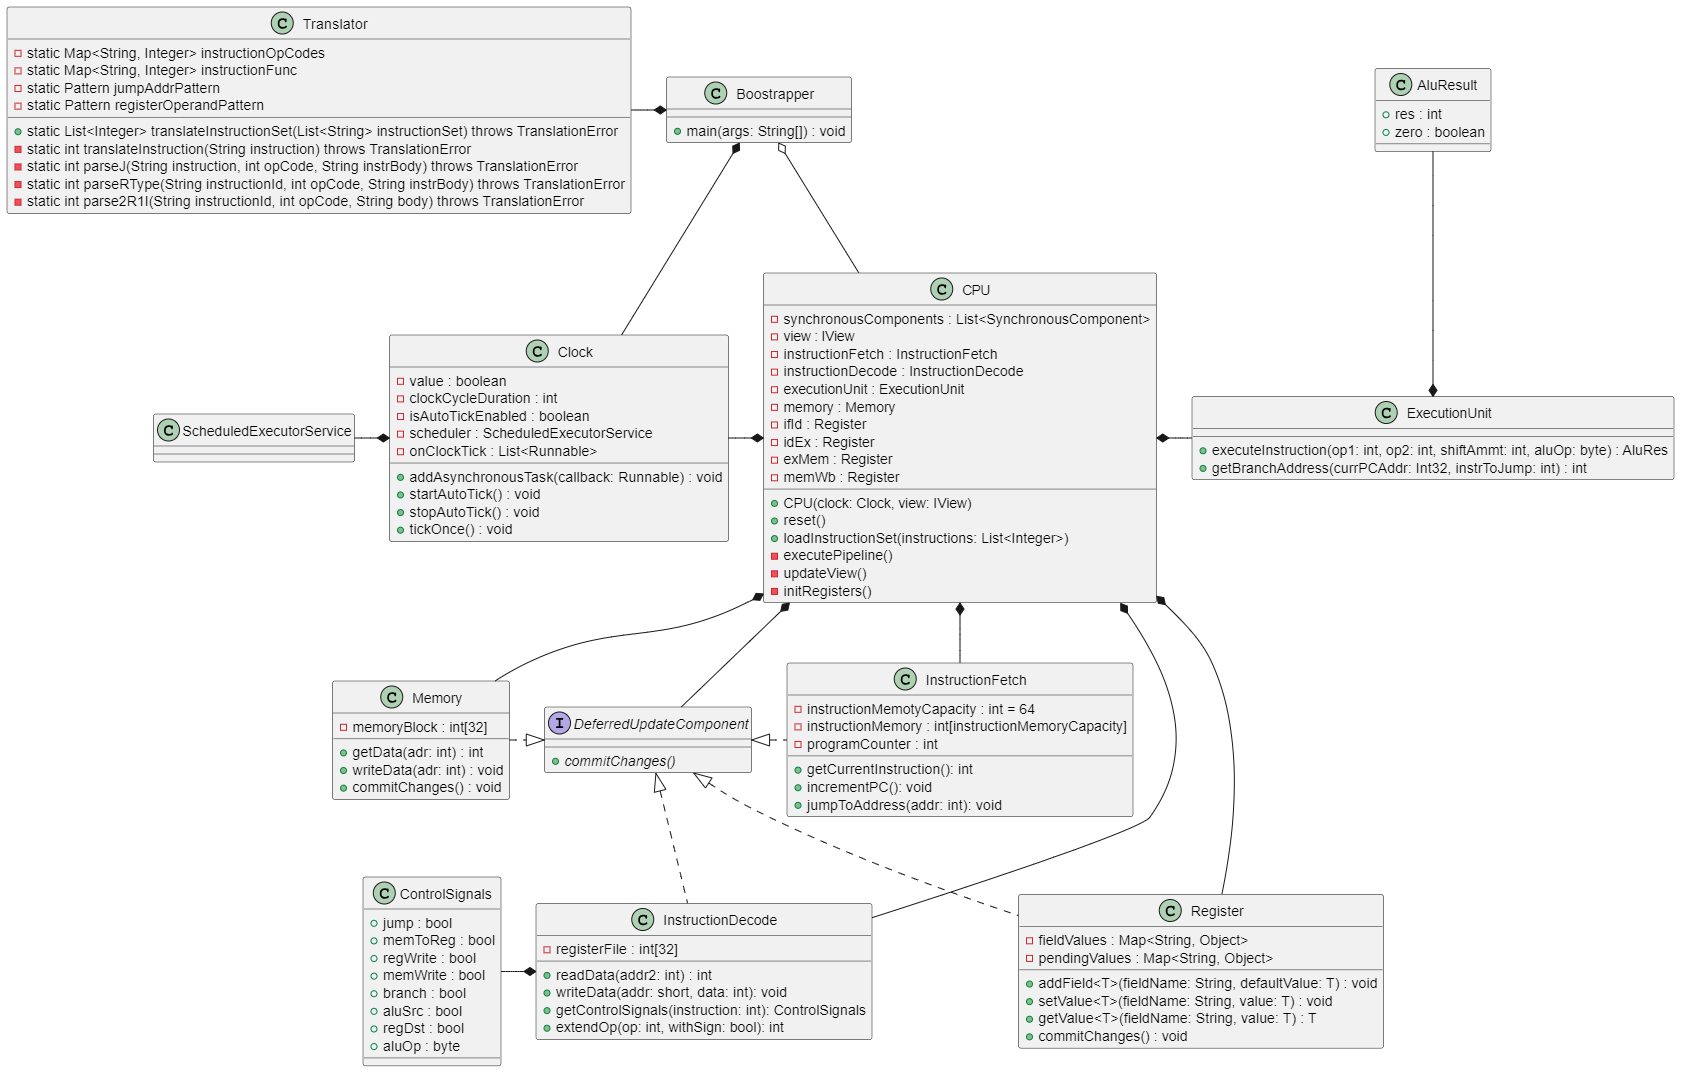
\includegraphics[width=\linewidth]{img/classDiagram.png}
\end{tcolorbox}

\subsubsection{Simularea registrelor inter-etaje}
Pentru simularea registrelor ce se află între etajele pipeline-ului, se folosește clasa \texttt{Register}. Clasa pune la dispoziție metode pentru manipularea convenabilă a conținutului. Metodele accesoare \texttt{getValue} și \texttt{setValue} sunt folosite pentru actualizarea și citirea valorilor din registru, în timp ce metoda generică \texttt{addField} e pentru a adăuga câmpuri noi de date în cadrul registrului, ceea ce permite refolosirea componentei pentru toate registrele necesare arhitecturii.

În interior, metoda \texttt{getValue} va actualiza valoarea curentă doar la finalul fiecărui ciclu de ceas pentru a facilita simularea unui comportament concurent. Astfel, toate apelurile de citire ale unei variabile din registru vor returna valoarea așteptată la acel moment. Pentru acesta, clasa va folosi două obiecte de tip \texttt{Map}, unul ce menține valorile actuale, iar, al doilea, ce menține valorile ce trebuie scrise la finalul ciclului, făcându-se un transfer între acestea. Pentru ca transferul să se realizeze în mod independent, clasa implementează interfața \texttt{DeferredUpdateComponent}. 



\subsubsection{CPU}
Această clasă reprezintă locul de îmbinare a tuturor sub-componentelor simulatorului, stocând instanțe pentru fiecare dintre ele și formează legăturile dintre acestea. De asemenea, "cunoaște" ordinea de execuție a instrucțiunilor și execută funcționalitățile expuse de sub-componente pentru prelucrarea lor în pipeline. De asemenea, menține o listă de componente ce implementează \texttt{DeferredUpdateComponent}.


La rularea aplicației, clasa înscrie pentru execuție pe semnalul de ceas toate operațiile și sarcinile care depind de acesta, precum execuția funției principale \texttt{executePipeline} și rularea funcției \texttt{update} a instanțelor ce implementează \texttt{DeferredUpdateComponent}. 

\subsubsection{Clock}
Clasa \texttt{Clock} este responsabilă de simularea semnalului de ceas și menține informații despre evenimentele care sunt înregistrate să se execute pe fiecare semnal de ceas. Modul de funcționare detaliat va fi descris în cele ce urmează.

\subsubsection*{Execuția sarcinilor}
Pentru execuția sincronă a sarcinilor în funcție de semnalul de ceas, se menține o listă cu obiecte de tip \texttt{Runnable}, care conține evenimentele ce trebuie să fie executate pe fiecare puls al semnalului de ceas. Valoare acestora este setată din exterior, prin intermediul metodelor accesoare aferente, iar ordinea de execuție a sarcinilor este cea a în care acestea au fost înscrise în listă.

Sunt posibile două moduri de execuție, selectabile de către utilizator, descrise și anterior la secțiunea \ref{subsec:ui}. Daca modul de execuție selectat este cel automat, se folosește un obiect de tip \texttt{ScheduledExecutorService} pentru rularea în buclă infinită a semnalului de ceas, până la primirea comenzii de oprire.

\begin{multicols}{2}
    \begin{tcolorbox}[colback=white!5!white,colframe=violet!75!black,title=Execuție tact cu tact]
        \begin{center}
            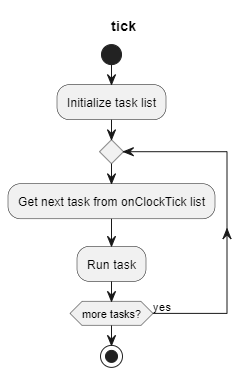
\includegraphics[width=.75\linewidth]{img/activityClockTick.png}
        \end{center}
    \end{tcolorbox}
    \columnbreak
    \begin{tcolorbox}[colback=white!5!white,colframe=violet!75!black,title=Execuție continuă]
        \begin{center}
            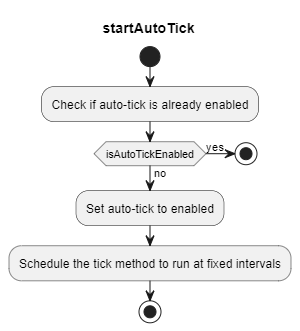
\includegraphics[width=.75\linewidth]{img/activityClockStartAutoTick.png}
        \end{center}
    \end{tcolorbox}
\end{multicols}

\subsubsection{InstructionFetch}
Componenta \texttt{InstructionFetch} este responsabilă de procurarea instrucțiunii curente din memoria de instrucțiuni și trimiterea acesteia la următorul etaj. Aici se află memoria de instrucțiuni, sub forma unui vector de lungime variabilă ce conține elemente de tip întregi pe 32 de biți, și numărătorul de program ce este stocat intr-o variabilă întreg pe 32 de biți. Componenta expune metode pentru acoperirea tuturor atribuțiilor pe care le îndeplinește.

\subsubsection{InstructionDecode}
Această clasă este locul unde se află fișierul de registre \texttt{Register File}. Rolul acesteia este de a decodifica instrucțiunea primită de la etajul anterior ca un întreg pe 32 de biți, de a genera semnalele de control, de a manipula \texttt{RF} și de extindere a operanzilor. Se folosesc hărțile de biți de la secțiunea \ref{subsec:instr} pentru a redirecționa bucățile relevante din instrucțiune către locul unde sunt procesate. Pentru gestionarea eficientă și intuitivă a semnalelor de control, se folosește o clasă suplimentară \texttt{ControlSignals} care va menține ca variabile membre toate semnalele de control necesare, prezente în arhitectura procesorului. 

Pentru a obține operanzii solicitați din \texttt{Register File} în funcție de adresele specificate în codul mașină al instrucțiunii, se folosește funcția \texttt{int readData(int addr)} care acceptă ca unic parametru adresa de la care se dorește citirea ca întreg pe 32 de biți și returnează datele din registrul adresat ca întreg pe 32 de biți. Aceasta se cheamă de două ori, o data folosind biții \texttt{[25:21]} din instrucțiune, iar apoi cu biții \texttt{[20:16]}, reprezentând adresele celor 2 operanzi. 

Semnalele de control se obțin folosind funcția \texttt{getControlSignals}, utilizând ca argument instrucțiunea în cod mașină. Funcția folosește un obiect de tip \texttt{Map} care memorează semnalele ce trebuie generate pentru fiecare tip de instrucțiune, interpretând câmpurile \texttt{OpCode} și \texttt{Func} ca chei.

\begin{tcolorbox}[colback=white!5!white,colframe=violet!75!black,title=Maparea semnalelor de control]
% Please add the following required packages to your document preamble:
% \usepackage[table,xcdraw]{xcolor}
% Beamer presentation requires \usepackage{colortbl} instead of \usepackage[table,xcdraw]{xcolor}
\begin{tabularx}{\linewidth}{ |l|X|X|X|X|X|X|X|}
\hline
\rowcolor{violet!75!black} \textcolor{white}{Instruction}  & \textcolor{white}{OpCode} & \textcolor{white}{Func} & \textcolor{white}{RegDst} & \textcolor{white}{ExtOp} & \textcolor{white}{AluSrc} & \textcolor{white}{Beq} & \textcolor{white}{Bgtz} \\
\hline
\rowcolor{violet!20!white} add & 000000 & 000000 & 1 & 0 & 0 & 0 & 0 \\
\hline
sub & 000000 & 000001 & 1 & 0 & 0 & 0 & 0 \\
\hline
\rowcolor{violet!20!white} sll & 000000 & 000010 & 1 & 0 & 0 & 0 & 0 \\
\hline
srl & 000000 & 000011 & 1 & 0 & 0 & 0 & 0 \\
\hline
\rowcolor{violet!20!white} and & 000000 & 000100 & 1 & 0 & 0 & 0 & 0 \\
\hline
or & 000000 & 000101 & 1 & 0 & 0 & 0 & 0 \\
\hline
\rowcolor{violet!20!white} xor & 000000 & 000110 & 1 & 0 & 0 & 0 & 0 \\
\hline
addi & 100000 & N/A & 0 & 1 & 1 & 0 & 0 \\
\hline
\rowcolor{violet!20!white} subi & 100001 & N/A & 0 & 1 & 1 & 0 & 0 \\
\hline
lw & 100010 & N/A & 0 & 1 & 1 & 0 & 0 \\
\hline
\rowcolor{violet!20!white} sw & 100011 & N/A & 0 & 1 & 1 & 0 & 0 \\
\hline
beq & 000010 & N/A & 0 & 1 & 0 & 1 & 0 \\
\hline
\rowcolor{violet!20!white} bgtz & 000100 & N/A & 0 & 1 & 0 & 1 & 1 \\
\hline
bne & 000011 & N/A & 0 & 1 & 0 & 1 & 0 \\
\hline
\rowcolor{violet!20!white} j & 000001 & N/A & 0 & 0 & 0 & 0 & 0 \\ 
\hline
\end{tabularx}

\vspace{1em}

\begin{tabularx}{\linewidth}{ |l|l|l|l|l|X|X|X|l|}
\rowcolor{violet!75!black} \textcolor{white}{Instruction}  & \textcolor{white}{OpCode} & \textcolor{white}{Func} & \textcolor{white}{bne} & \textcolor{white}{Jmp} & \textcolor{white}{MemWrite} & \textcolor{white}{MemToReg} & \textcolor{white}{RegWrite} & \textcolor{white}{AluOp} \\
\hline
\rowcolor{violet!20!white} add & 000000 & 000000 & 0 & 0 & 0 & 0 & 1 & 0000 \\
\hline
sub & 000000 & 000001 & 0 & 0 & 0 & 0 & 1 & 0000 \\
\hline
\rowcolor{violet!20!white} sll & 000000 & 000010 & 0 & 0 & 0 & 0 & 1 & 0000 \\
\hline
srl & 000000 & 000011 & 0 & 0 & 0 & 0 & 1 & 0000 \\
\hline
\rowcolor{violet!20!white} and & 000000 & 000100 & 0 & 0 & 0 & 0 & 1 & 0000 \\
\hline
or & 000000 & 000101 & 0 & 0 & 0 & 0 & 1 & 0000 \\
\hline
\rowcolor{violet!20!white} xor & 000000 & 000110 & 0 & 0 & 0 & 0 & 1 & 0000 \\
\hline
addi & 100000 & N/A & 0 & 0 & 0 & 0 & 1 & 0001 \\
\hline
\rowcolor{violet!20!white} subi & 100001 & N/A & 0 & 0 & 0 & 0 & 1 & 0010 \\
\hline
lw & 100010 & N/A & 0 & 0 & 0 & 1 & 1 & 0011 \\
\hline
\rowcolor{violet!20!white} sw & 100011 & N/A & 0 & 0 & 1 & 0 & 0 & 0100 \\
\hline
beq & 000010 & N/A & 0 & 0 & 0 & 0 & 0 & 0101 \\
\hline
\rowcolor{violet!20!white} bgtz & 000100 & N/A & 0 & 0 & 0 & 0 & 0 & 0110 \\
\hline
bne & 000011 & N/A & 1 & 0 & 0 & 0 & 0 & 0111 \\
\hline
\rowcolor{violet!20!white} j & 000001 & N/A & 0 & 1 & 0 & 0 & 0 &1000 \\
\hline
\end{tabularx}
\end{tcolorbox}

\subsubsection{ExecutionUnit}
Componenta \texttt{ExecutionUnit} reprezintă unitatea aritmetico-logică a procesorului \texttt{ALU} și încapsulează logica responsabilă de generarea rezultatului \texttt{ALU} în funcție de semnalul \texttt{AluOp}.

\subsubsection{Memory}
Clasa \texttt{Memory} simulează etajul cu același nume al pipeline-ului, și este responsabilă cu stocarea conținutului memoriei de date a procesorului (\texttt{memoria RAM}). Deoarece este, practic, o componentă sincronă cu stare, în cadrul simulatorului aceasta implementează interfața \texttt{DeferredUpdateComponent}. Aceasta are o capacitate fixă redusă pentru scopul simulării, dar există opțiunea ca pe viitor sa poată fi modificată de către utilizator cu ajutorul interfeței grafice. Expune metode pentru manipularea conținutului memoriei.


\subsubsection{WritebackUnit}
Etajul \texttt{WriteBack} nu corespondează unei componente software concrete a simulatorului din cauza complexității relativ mici a acestuia, astfel funcționalitatea ce îi corespunde fiind implementată direct în componenta \texttt{CPU}. Are scopul de a transmite informațiile din ultimul registru inter-etaj către componentele relevante.

\subsection{Translatorul din limbaj de asamblare în cod mașină}
Pentru conveniență, simulatorul acceptă ca input instrucțiuni în limbaj de asamblare, descrise în Secțiunea~\ref{subsec:instr}. Astfel, apare necesitatea unui utilitar care să valideze și traducă șiruri de caractere introduse de utilizator de la tastatură. Clasa \texttt{Translator} va pune la dispoziție celorlalte module ale aplicației funcții de traducere și validare, prezentate în cele ce urmează.


Ca arhitectură, aceasta va menține \texttt{map}-uri corelarea unui tip de instrucțiune spre \texttt{opcode}-ul sau codul \texttt{func} corespunzător. De asemenea, va memora expresii regex pentru folosirea validarea formatului operanzilor.

\begin{tcolorbox}[colback=white!5!white,colframe=violet!75!black,title=Diagramă de clasa - Translator]
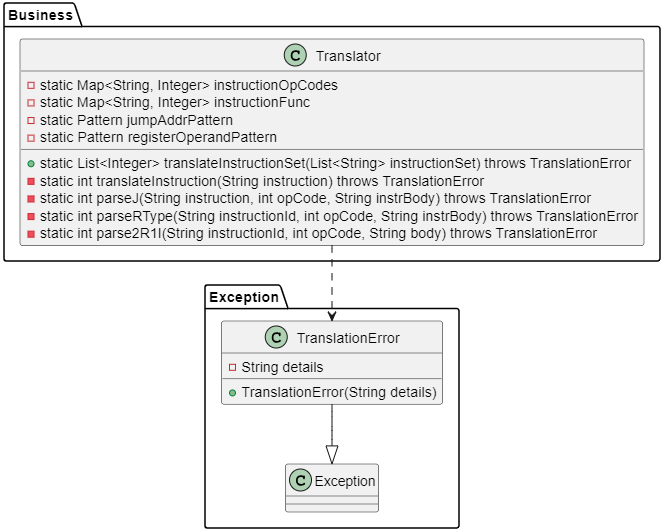
\includegraphics[width=\textwidth]{img/classTranslator.png}
\end{tcolorbox}

Clasa expune o singură metodă publică, \texttt{translateInstructionSet}, care acceptă o listă de instrucțiuni în limbaj de asamblare ca parametru și returnează o listă de întregi, simbolizând instrucțiunile traduse. Această metoda va apela în buclă metoda privata \texttt{translateInstruction}, pentru a încerca să traduca, pe rând, instrucțiunile. Modul de operare poate fi observat în diagrama de mai jos.

\begin{tcolorbox}[colback=white!5!white,colframe=violet!75!black,title=Diagramă de clasa - Translator]
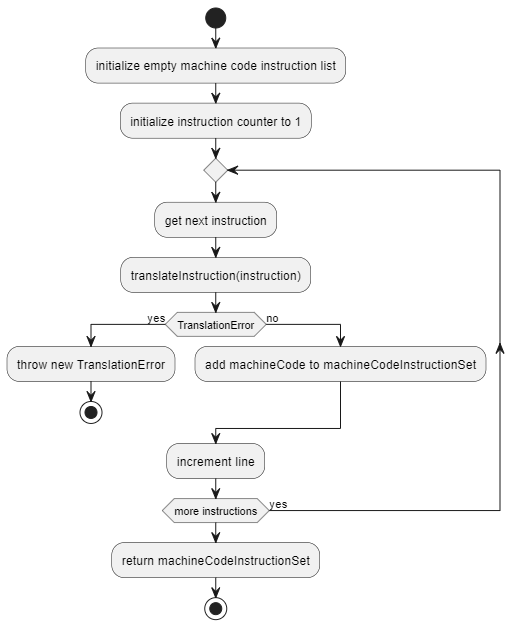
\includegraphics[width=\textwidth]{img/activityTranslateInstructionSet.png}
\end{tcolorbox}

Funcția \texttt{translateInstruction}, la rândul ei, se folosește de alte 3 metode ajutătoare pentru a organiza logica în funcție de tipul instrucțiunii curente. Astfel, pentru instrucțiuni de tip R cu 3 operanzi de tip registru se va apela \texttt{parseRType}, de instrucțiuni de tip I se va ocupa funcția \texttt{parse2R1I}, iar instrucțiunea J va fi tradusă cu ajutorul \texttt{parseJType}.

\begin{tcolorbox}[colback=white!5!white,colframe=violet!75!black,title=Diagramă de clasa - Translator]
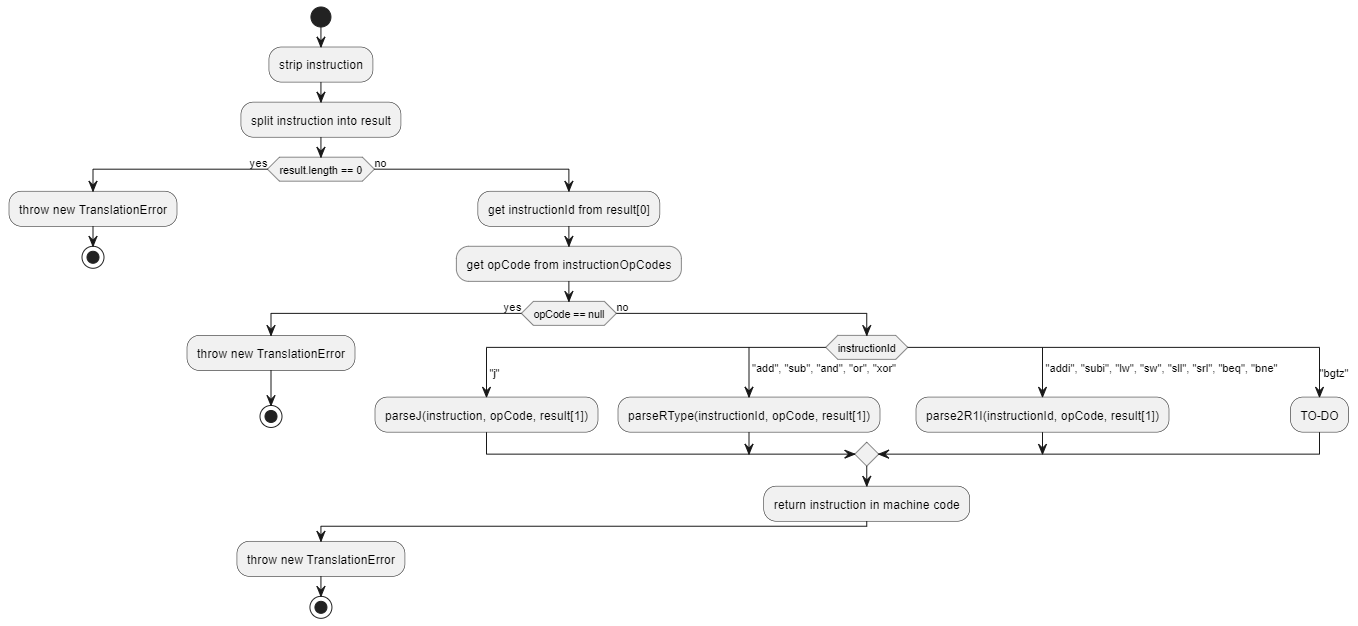
\includegraphics[width=\textwidth]{img/activityParseInstruction.png}
\end{tcolorbox}

\subsection{Interfață grafică}
Interfața grafică este implementată folosind tehnologii web, datorită versatilității pe care le oferă, suportului extensiv și multitudinea de librării disponibile. Astfel, concret, interfața grafică este scrisă folosind framework-ul de Javascript Next.js, portofoliul CSS Tailwind pentru stilizare.

Interfața grafică include schema bloc a procesorului MIPS Pipeline, în care sunt vizibile componentele principale, precum \texttt{Register File}, memoria de instrucțiuni sau registrele inter-etaj, împreună cu conținuturile lor. Totodata, semnalele mai relevante sunt afișate în mod interactiv, fiind colorate diferit în funcție de valoarea acestora (high/low).

De asemenea, interfața include și un meniu de opțiuni de unde utilizatorul poate declanșa execuția unui semnal de ceas, resetarea execuției unui program încarcat, sau încărcarea unui program nou sub forma unui set de instrucțiuni assembly, care sunt validate de erori și traduse, mai apoi, în cod mașină suportat de simulator.

\begin{tcolorbox}[colback=white!5!white,colframe=violet!75!black,title=Design interfață grafică]
    \begin{center}
        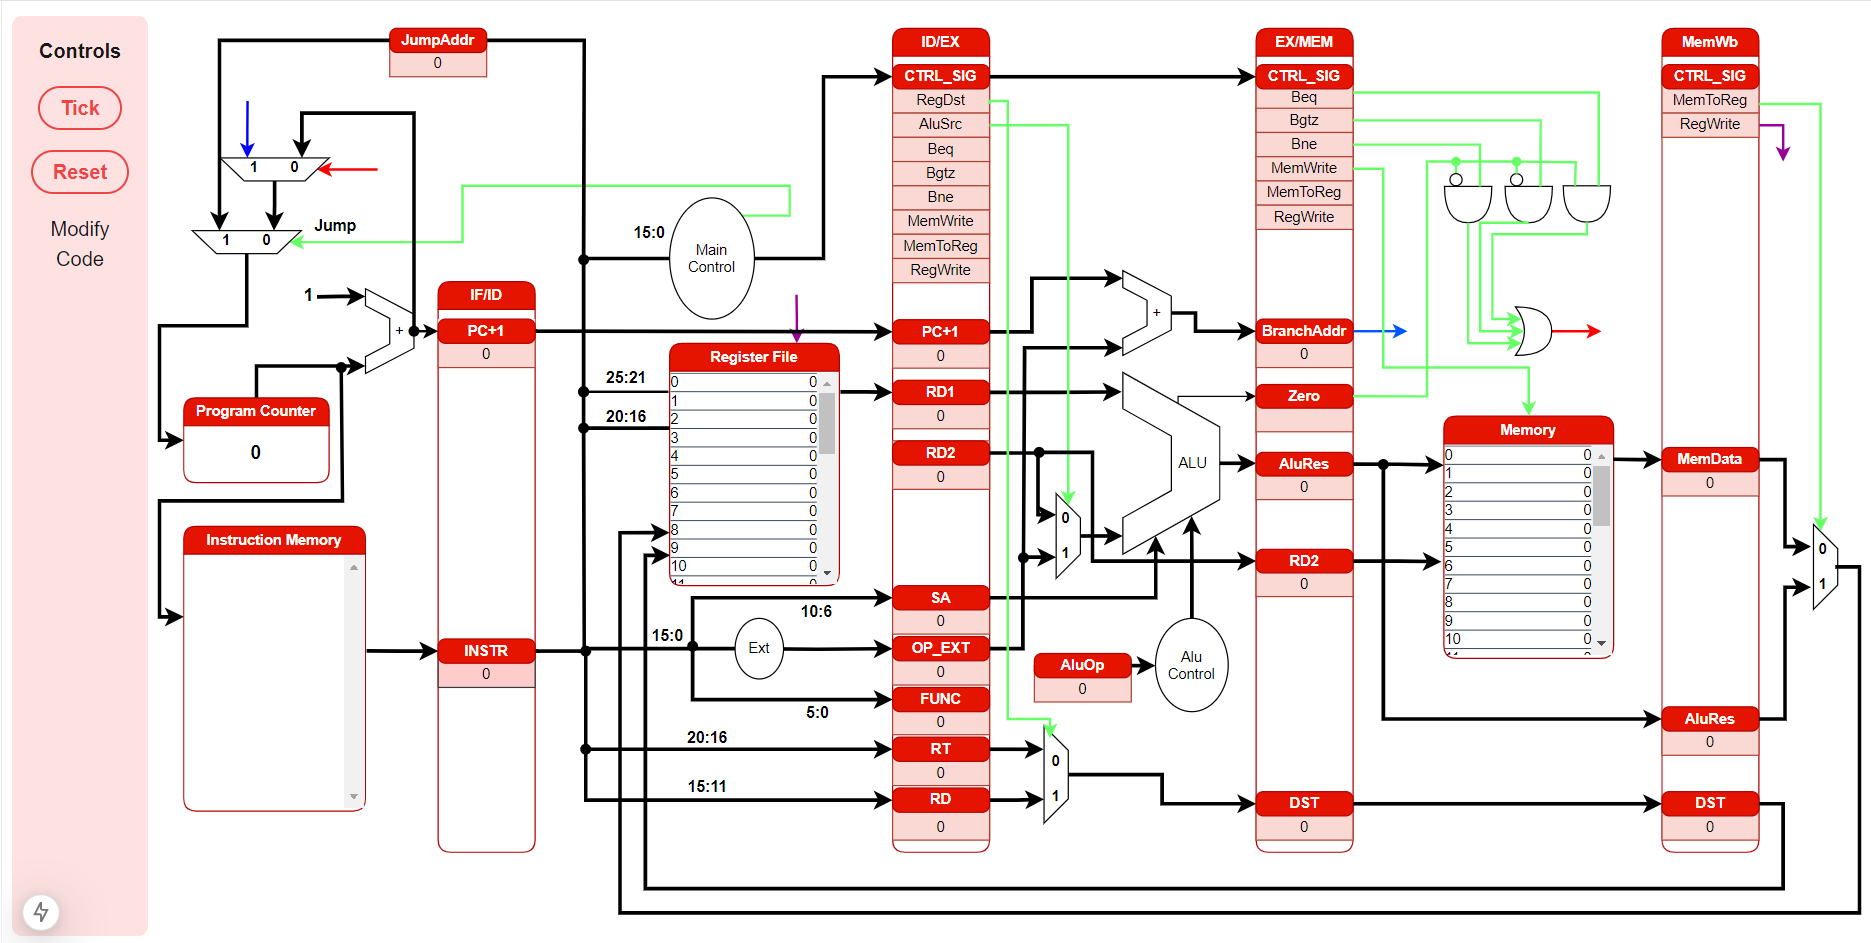
\includegraphics[width=\textwidth]{img/ui_ss.png}
    \end{center}
\end{tcolorbox}

\newpage

\section{Implementare}

\subsection{Arhitectură generală - clasa \texttt{CPU}}
Componenta principală a simulatorului este clasa \texttt{CPU}. Aceasta încapsulează și inițializează tot restul componentelor. 

Funcția \texttt{executePipeline} descrie execuția pipeline-ului într-un ciclu de ceas. 

\subsubsection{Etapa Instruction Fetch}
În etapa ce corespunde etajului Instruction Fetch, se extrage instrucțiunea curentă și valoarea următoare a contorului de program din instanța componentei \texttt{InstructionFetch}, iar, mai apoi, se înscriu aceste valori  spre actualizare în registrul IF/ID.

\begin{javacodebox}[Etajul If]
ifId.setValue(INSTRUCTION, instructionFetch.getInstruction());
instructionFetch.incrementProgramCounter();
ifId.setValue(PROG_CNT, instructionFetch.getProgramCounter());
\end{javacodebox}

\subsubsection{Etapa Instruction Decode}
În această etapă, se extrage din registrul IF/ID codul instrucțiunii și PC+1 (contorul de program urmator la momentul când acesta a intrat în pipeline).
Se extrag cele 2 valori de adresă din codul instrucțiunii folosind operații pe biți și se verifică dacă nu cumva instrucțiunea curentă este una de salt. De asemenea, se calculează valorile semnalelor de control.

\begin{javacodebox}[Cod sursă - Decodificare valori din instrucțiune]
int instrId = ifId.getValue(INSTRUCTION, Integer.class);
ControlSignals idCtrlSig = instructionDecode.getControlSignals(instrId);
int addr1 = (instrId >> 21) & 0x1f;
int addr2 = (instrId >> 16) & 0x1f;

if(idCtrlSig.getSignalValue(ControlSignals.Signals.Jmp)) {
    int jumpAddr = instrId & 0x0000FFFF;
    instructionFetch.jumpToAddress(jumpAddr);
}
\end{javacodebox}

Se verifică dacă trebuie scrise date venite din etajul Write Back în fișierul de registre.

\begin{javacodebox}[Cod sursă - Verificare scriere RF]
boolean regWrite = memWb.getValue(CTRL_SIG, ControlSignals.class).getSignalValue(ControlSignals.Signals.RegWrite);
if(regWrite)
{
    int data = memWb.getValue(CTRL_SIG, ControlSignals.class).getSignalValue(ControlSignals.Signals.MemToReg)
            ? memWb.getValue(MEM_DATA, Integer.class)
            : memWb.getValue(ALU_RES, AluRes.class).res;
    int regAddr = memWb.getValue(REG_DST, Integer.class);
    instructionDecode.writeData(regAddr, data);
}
\end{javacodebox}

În cele din urmă, se scrie registrul ID/EX cu valorile corespunzătoare.

\begin{javacodebox}[Cod sursă - Scriere ID/EX]
idEx.setValue(CTRL_SIG, idCtrlSig);
idEx.setValue(PROG_CNT, ifId.getValue(PROG_CNT, Integer.class));
idEx.setValue(RD1, instructionDecode.readData(addr1));
idEx.setValue(RD2, instructionDecode.readData(addr2));
idEx.setValue(SHIFT_AMM, (instrId >> 6) & 0x1f);
idEx.setValue(EXT_OP, instructionDecode.extendOp(instrId & 0xffff, idCtrlSig.getSignalValue(ControlSignals.Signals.ExtOp)));
idEx.setValue(FUNC, instrId & 0x3f);
idEx.setValue(REG_TGT, (instrId >> 16) & 0x1f);
idEx.setValue(REG_DST, (instrId >> 11) & 0x1f);
\end{javacodebox}

\subsubsection{Etapa \textit{Execution}}
În etapa de execuție este folosită instanța clasei \texttt{ExecutionUnit} pentru a efectua operațiile necesare pe operanzi, în funcție de semnalele \texttt{func} și \texttt{AluOp}. De asemenea, aici se calculează și adresa de ramificare.
Mai întâi, sunt obținute datele din registrul IF/ID și se decide care dintre acestea vor reprezenta sursa pentru operanzii ce urmează a fi folosiți. 

\begin{javacodebox}[Cod sursă - Obținerea operanzilor]
int extOp = idEx.getValue(EXT_OP, Integer.class);
int exOp1 = idEx.getValue(RD1, Integer.class);
int exOp2 = exCtrlSig.getSignalValue(ControlSignals.Signals.AluSrc)
    ? extOp
    : idEx.getValue(RD2, Integer.class);
int shiftAmm = idEx.getValue(SHIFT_AMM, Integer.class);
int func = idEx.getValue(FUNC, Integer.class);
\end{javacodebox}

Tot în această etapă se decide care va fi registrul destinație trimis către și utilizat în etapa de \textit{write-back}.

\begin{javacodebox}[Cod sursă - Determinarea registrului destinație]
int finalRegDst = exCtrlSig.getSignalValue(ControlSignals.Signals.RegDst)
    ? idEx.getValue(REG_DST, Integer.class)
    : idEx.getValue(REG_TGT, Integer.class);
\end{javacodebox}

În cele din urmă, se scriu datele în registrul EX/MEM.

\begin{javacodebox}[Cod sursă - Calcularea și scrierea adresei de ramificare în registrul EX/MEM]
exMem.setValue(BRANCH_ADDR, exProgCnt + extOp);
\end{javacodebox}

\begin{javacodebox}[Cod sursă - Scrierea celorlaltor valori în EX/MEM]
exMem.setValue(CTRL_SIG, exCtrlSig);
exMem.setValue(ALU_RES, executionUnit.executeInstruction(exOp1, exOp2, shiftAmm, exCtrlSig.aluOp, (byte)func));
exMem.setValue(RD2, idEx.getValue(RD2, Integer.class));
exMem.setValue(REG_DST, finalRegDst);
\end{javacodebox}

\subsubsection{Etapa \textit{Memory}}
Porțiunea din metodă corespunzătoare etapei \textit{Memory} împachetează logica responsabilă de procurarea datelor din memoria ram și de scrierea de date în aceasta. Totodată, aici se ia decizia de ramificare în cazul instrucțiunilor de \textit{branch}.

Pentru manipularea memoriei, se obțin eventuala adresă calculată în etapa precedentă și semnalele de control din registrul EX/MEM. În cazul în care semnalul de control \texttt{MemWrite} este setat, se va scrie datele în memorie la această adresă, în caz contrar, se vor citi datele de la adresă și se vor scrie în registrul MEM/WB.

\begin{javacodebox}[Cod sursă - Manipularea condițională a memoriei]
ControlSignals memCtrlSig = exMem.getValue(CTRL_SIG, ControlSignals.class);
AluRes memAluRes = exMem.getValue(ALU_RES, AluRes.class);
int memAddr = memAluRes.res & 0x000000FF; // RAM capacity limited at 256 * 4 bytes for simulation purposes
if(memCtrlSig.getSignalValue(ControlSignals.Signals.MemWrite))
{
    System.out.println("Addr: " + memAluRes.res + "; Data: " + exMem.getValue(RD2, Integer.class));
    memory.writeData(memAddr, exMem.getValue(RD2, Integer.class));
}
else
{
    memWb.setValue(MEM_DATA, memory.readData(memAddr)); 
}
\end{javacodebox}

Decizia de salt se ia în funcție de semnalele de salt \texttt{Beq}, \texttt{Bne}, \texttt{Bgtz} și rezultatele produse de componenta \texttt{ExecutionUnit} în stagiul precedent - indicatorul de nul \texttt{Zero} și \texttt{AluRes}.

\begin{javacodebox}[Cod sursă - Luarea deciziei de salt]
if (memCtrlSig.getSignalValue(ControlSignals.Signals.Beq) && memAluRes.zero ||
    memCtrlSig.getSignalValue(ControlSignals.Signals.Bne) && !memAluRes.zero ||
    memCtrlSig.getSignalValue(ControlSignals.Signals.Bgtz) && memAluRes.res > 0
) {
    int branchAddr = exMem.getValue(BRANCH_ADDR, Integer.class);
    instructionFetch.jumpToAddress(branchAddr);
}
\end{javacodebox}

\par{}

\newpage
\section{Bibliography}
[1] Cristian Vancea, Arhitectura Calculatoarelor - Indrumator de Laborator: https://users.utcluj.ro/~vcristian/Indrumator\_laborator\_2024\_Draft.pdf

[2] Java SE 8 Documentation: https://docs.oracle.com/javase/8/docs/api/

[3] Geeks for Geeks: www.geeksforgeeks.org
 
\end{document}
